The final day of the regular conference!

\subsection{Contributed Talks: RL}

We begin with the final RL session.


\subsubsection{Batch Policy learning under Constraints~\cite{le2019batch}}

Talk by Hoang M. Le. \\

{\bf Motivation}:
\begin{enumerate}
    \item {\it Change RL Objective:} Consider usual RL objective:
    \[
    \min_x C(\pi) = \bE\left[\sum cost(s,a)\right]
    \]
    But, in reality, not always feasible. $\ra$ Hard to define a single cost function!
    
    $\therefore$ Specifying additional constraints seems naturak.
    
    \item {\it Sample Efficient Batch RL:} But, if we change the cost objective, we need to solve a new problem that can make RL even harder.
    
    $\ra$ In batch RL, tend to think about having some existing data set (from some prior policy, $\pi_D$, that may be sub-optimal). \\
    
    Q1: Can we use this abundant source of data to learn a better, new policy?
    
    Q2: What if we want to change our constraints? Can we still learn a new policy under these new constraints?
\end{enumerate}

Notation:
\begin{itemize}
    \item Data set of $n$ tuples of data, $D = \{(s,a,r,s'), \ldots$, generated by $\pi_D$.
    \item Goal is to find some $\pi$ such that $\min_\pi C(\pi)$, subject to some constraint $G(\pi) \leq 0$.
\end{itemize}

Examples: 1) Counterfactual and safe policy learning (constraint specifies to avoid certain states), or 2) Multi-criteria value-based constraints (driving, minimize travel time subject to constraint that we stay in a particular lane). \\

{\bf Problem:} Lagrangian:
\[
L(\pi, \lambda) = C(\pi) + \lambda^\top G(\pi),
\]
where the primal is: 
\[
\min_\pi \max_{\lambda \geq 0} L(\pi, \lambda)
\]
and the dual is:
\[
\max_{\lambda \geq 0} \min_\pi L(\pi, \lambda).
\]

Thus: extend policy class to allow randomized policies to handle non-convex costs.

{\bf Approach:} Reductions to supervised learning and online learning. \\


{\bf Algorithm Sketch:} Repeat the following:
\begin{enumerate}
    \item $\pi \la$ Best-response$(\lambda)$, where this usually comes from Fitted Q-Iteration~\cite{ernst2005tree}.
    \item $L_{max} = $ evaluate (dual) fixing $\pi$
    \item $L_{min} = $ evaluate (primal) fixing $\lambda$
    \item If $L_{max} - L_{min} \leq \omega$, STOP.
    \item Otherwise, $\lambda \la$ Online-algorithm(all prior $\pi$).
\end{enumerate}

To handle the evaluation steps, rely on off-policy evaluation. That is: given $D$, want to estimate $\hat{C}(\pi) \approx C(\pi)$. \\

$\ra$ Propose a new model-free direct method for off-policy evaluation called Fitted Q Evaluation (FQE). Sketch:
\begin{enumerate}
    \item Choose a function class. Then, for $k$ iterations:
    \item Solve for $Q$ ; $(s,a) \mapsto y = c = Q_{prev}(s', \pi(s'))$
    \item $Q_{prev} \la Q$.
\end{enumerate}

\begin{theorem}
End-to-end guarantee for FQE: for $n = poly(1/\eps, \log 1/\delta, \log K, \ldots)$, with $\Pr 1-\delta$:
\[
|C(\pi) - \hat{C}(\pi)| \leq O(\omega +\sqrt{\beta}\eps),
\]
with $\omega$ a chosen stopping condition for FQE.
\end{theorem}

{\bf Experiments:} A top-down driving task with the goal of minimizing travel time, while satisfying constraints like smooth driving and staying in the center of a lane. Train on a $\pi_D$ that {\it ignores} these constraints. \\

$\ra$ Finding: output policy from the algorithm can satisfy the new constraints, while keeping performance high (travel time).

\spacerule


\subsubsection{Quantifying Generalization in RL~\cite{cobbe2018quantifying}}

Talk by Karl Cobbe. \\

{\bf Note:} Lots of deep RL algorithms use same tasks for training and testing. \\

$\ra$ So, this work introduces new environments designed to study generalization explicitly in deep RL. Better benchmarks $\implies$ Better research, better algorithms. \\

{\bf Maing Finding:} Lots of deep RL algorithms do in fact overfit on this environment (which is explicitly supposed force agents to generalixe well). \\

Coin run domain:
\begin{enumerate}
    \item 2D platformer, agent has to collect coins
    \item Level generation conditioned on difficulty
    \item Can construct training sets of arbitrary size.
\end{enumerate}

{\bf Benchmark Results:} Run a variety of architectures on tasks from the coin run domain (with a split train/test set). \\

$\ra$ Finding 1: Overfitting is in fact a significant problem

$\ra$ Finding 2: deeper architectures tend to generalize better (3 vs. 15 conv layers).

$\ra$ Finding 3: Explore different effects of regularization schemes like $L_2$, dropbout, batch norm, and data augmentation. They are all similarly effective at regularization. \\

Code: \url{github.com/openai/coinrun}

\spacerule

\subsubsection{Learning Latent Dynamics for Planning from Pixels~\cite{hafner2018learning}}

Talk by Danijar Hafner. \\

{\bf Problem:} Planning has been really effective when the world model is known (as in AlphaGo). But, it has proven ineffective with complex or unknown transitions. \\

$\ra$ Consider visual control tasks: MuJoCo but with images as input. \\

{\bf This Work:} PLaNet: 1) Recipe for scalade model-based RL, 2) Efficient planning in latent space with large batch size, 3) Significantly more sample efficient than model-free methods. \\

\begin{figure}
    \centering
    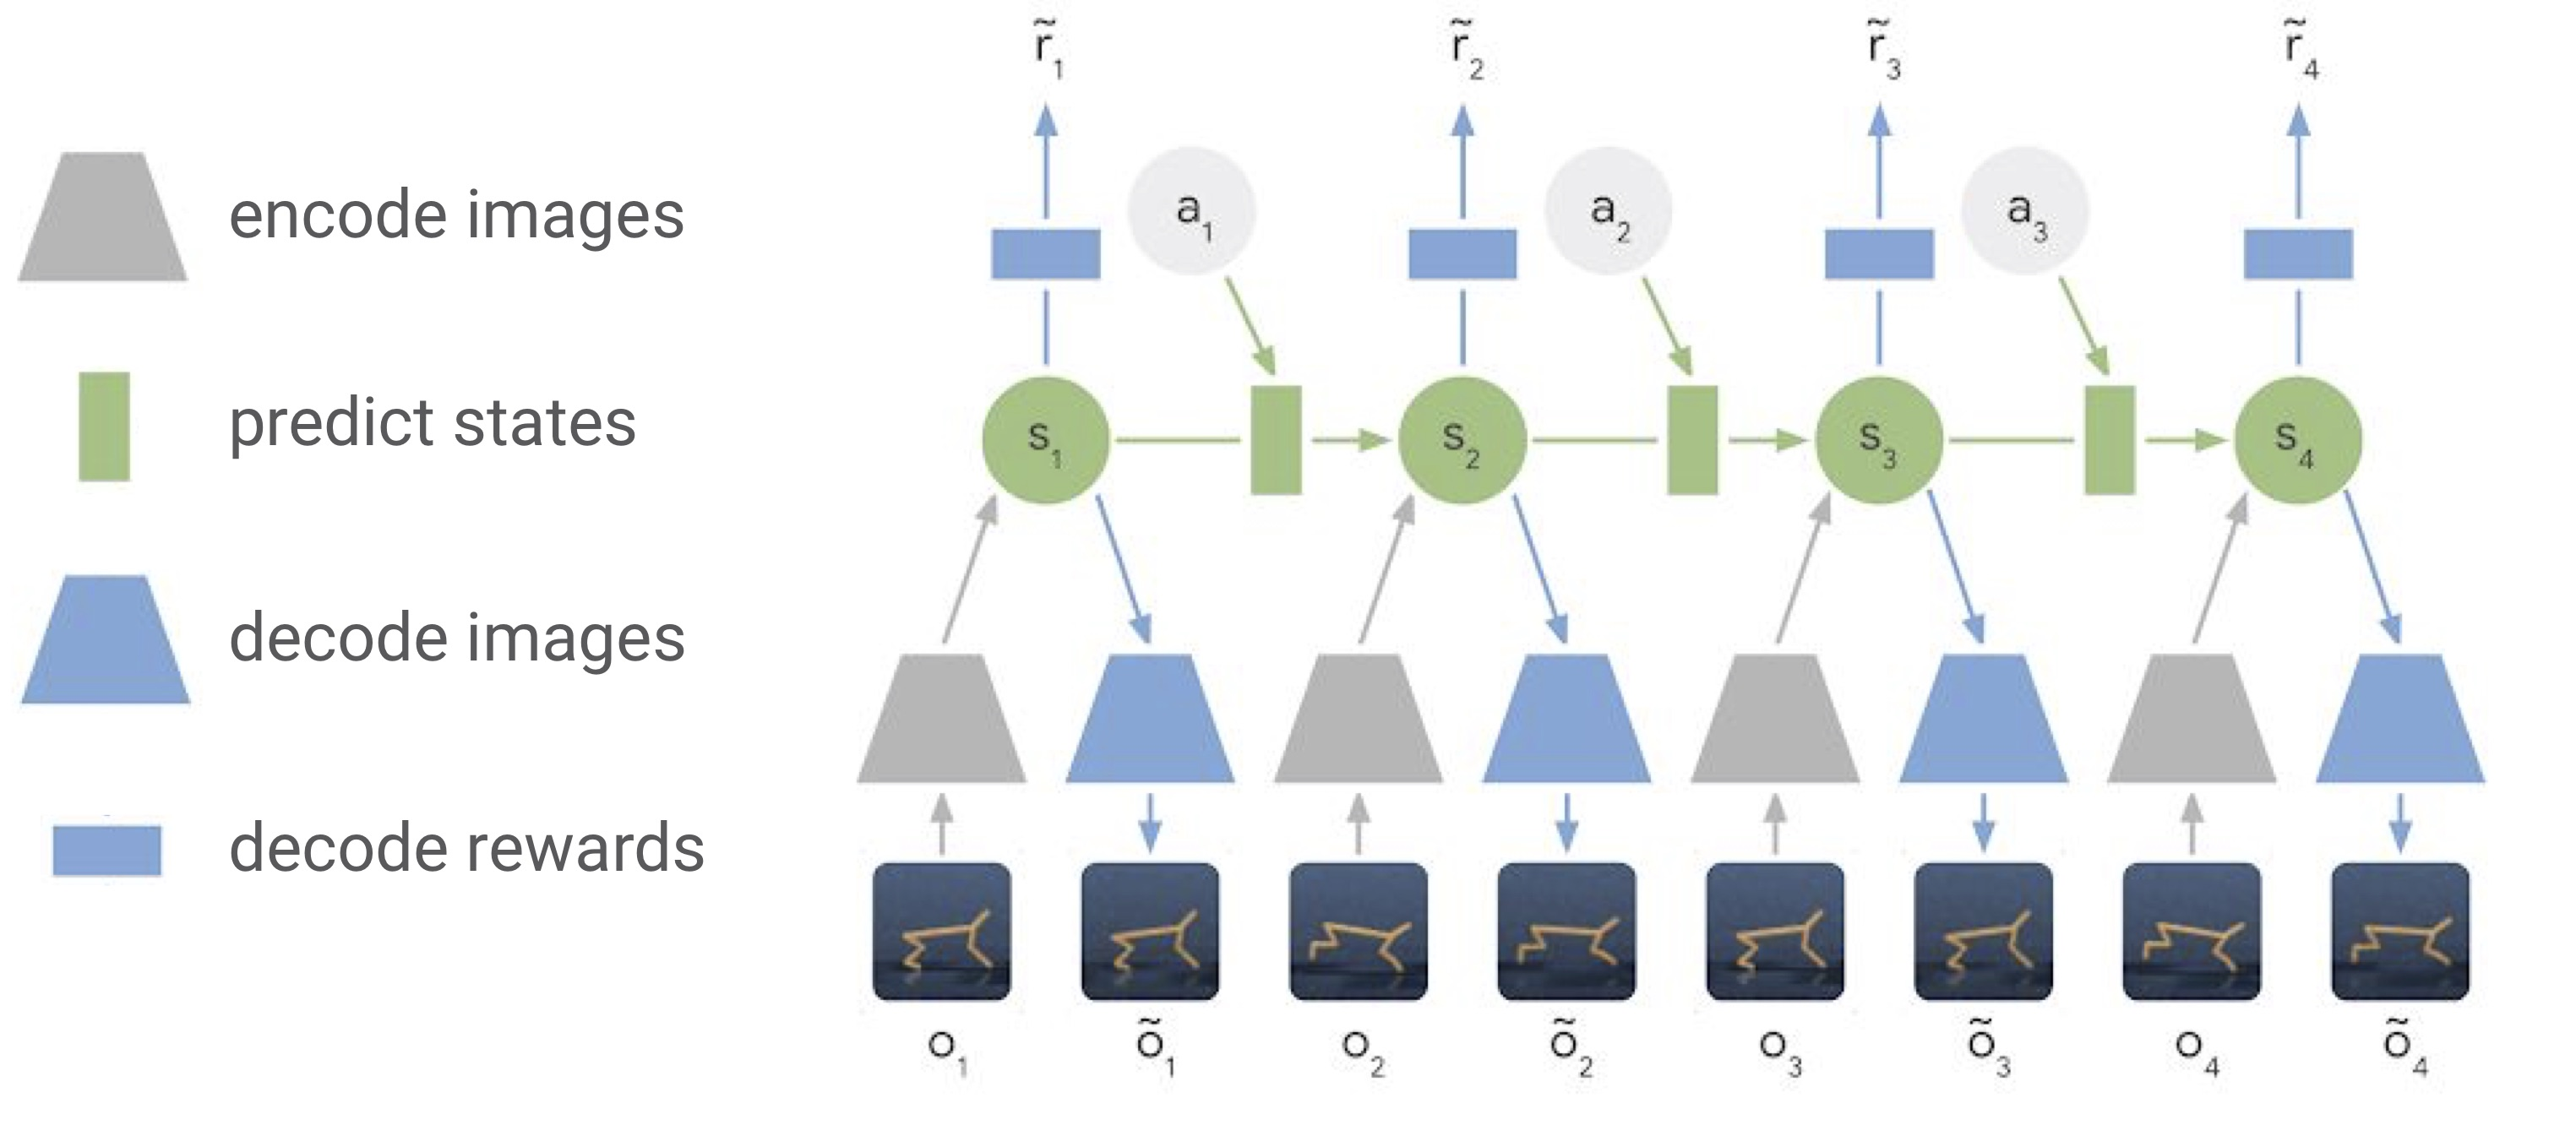
\includegraphics[width=0.45\textwidth]{images/planet.jpg}
    \caption{PLaNET latent dynamics model.}
    \label{fig:planet}
\end{figure}

{\bf Experiments:} Compare to model-free agents on visual variant of MuJoCo tasks, achieves competitive performance (to model-free methods) but with far fewer samples. \\

Thus: a scalable method for model-based RL in image space. \\

Code: \url{danijar.com/planet}

\spacerule

\subsubsection{Projections for Approximate Policy Iteration~\cite{akrour2019projections}}

Talk by Riad Akrour. \\

{\bf Consider:} Entropy regularization in RL is widespread with actor-critic methods (see: SAC, NAC, PPO, A3C, REPS, ACER, ACKTR, TRPO). \\

Soft constraint:
\[
max\pi_ J(\pi) + \alpha H(\pi).
\]
where $J$ is the objective (return) and $H$ is entropy. Conversely, the hard constraint:
\[
\max_\pi J(\pi)\ \text{ s.t. }\ H(\pi) \geq \beta
\]
$\ra$ Harder to optimize (the hard constraint), easier to tune.

{\bf Contributions:} 1) Project hard constraint of Shannon entropy of Gaussian or soft max policies, and 2) Perform projections of hard constraint, yields an optimization scheme for deep RL. \\

{\bf Experiment:} Compare different actor-critic/policy-optimization algorithms with entropy bonus vs. their projection-based method. \\
$\ra$ Entropy bonus is ineffective early on, but with a strict entropy constraint, yields better exploration and better policies. Simple scheme, can be incorporated into any RL algorithm. \\

\spacerule

\subsubsection{Learning Structured Decision Problems with Unawareness~\cite{innes2019learning}}

Talk by Craig Innes. \\

{\bf Focus:} ``Unawareness" in decision making.\\

$\ra$ Example: Farming. What might an agent learn? Dynamics between protein levels in grain, when and which grains to fertilize, and so on. \\

Q: But what if, part way through the problem, we discover new state variables and actions that are critical to performing optimally? \\

A: If we don't explicitly model this kind of unawareness, agents might not be able to solve many kinds of problems. \\

{\bf Contributions:} Agent learns an interpretable model of a decision problem incrementally via evidence from domain trials and expert advice.\\

$\ra$ Approach: if agent's performance in last $k$ trials is below threshold $\beta$ of true policy $\pi_+$, say: ``At time $t$ you should have done $a'$ rather than $a_t$." Agent can then learn lots from this feedback: 1) new action, 2) $a'$ has more value than $a_t$, and so on. \\

{\bf Experiments:} A suite of randomly generated decision problems. \\

$\ra$ Finding 1: New agent is able to learn the true optimal policy, despite starting unaware of state variables and actions. 
$\ra$ Finding 2: Varying experts tolerance of when to intervene has a profound impact on agent's learning capacity.

\spacerule
\subsubsection{Calibrated Model-Based Deep RL~\cite{malik2019calibrated}}

Talk by Ali Malik. \\

{\bf Consider:} Uncertainty is rampant in the real world. To make effective RL systems for the real world, we have to tackle this uncertainty head on. \\

%Overview: 1) Importance of uncertainty, 2) Which uncertainty matters in model-based RL? (MBRL), 3) Calibration and Recalibration, 4) Experiments/results. \\

$\ra$ Thus, important to model uncertainty accurately. \\

Q: What type of uncertainty is important to model in RL? \\

A: Turn to statistics! Consider meteorologists, for instance: adopt ``proper scoring rules", which are losses that hold when the predicted distribution matches the true distribution rules. \\

\ddef{Proper Scoring Rules}{A measurement for how well a model captures uncertainty based on two criteria:
\begin{enumerate}
    \item {\bf Sharpness:} Predictive distributions should be focused (have low variance)
    \item {\bf Calibration:} Uncertainty should be empirically accurate (about $p\%$ of the time I should be right, if I predict something as having a propensity of $p$).
\end{enumerate}}


{\bf CLaim:} Calibration in particular is really important for model-based RL. \\

Q: Why? \\

A1: For planning! Calibrated uncertainties lead o better estimates of expectation. 

\begin{theorem}
The value of $\pi$ for an MDP under true dynamics is equal to the value of the policy under a {\it calibrated} dynamics model $\widehat{T}$.
\end{theorem}

A2: For exploration! Many exploration/exploitation algorithms use upper confidence bounds (UCB) to guide choices such as LinUCB:
\[
\argmax_{a \in \mc{A}}\left(x \theta_a = \alpha \sqrt{x \hat{\Sigma}_a x}\right).
\]
Calibration naturally improves UCBs, resulting in better exploration. \\

Q: How do we make sure our systems have calibrated uncertainty? (note that deep networks' uncertainty is often uncalibrated) \\

A: Turn to method from prior work: {\it recalibration} from~\citet{kuleshov2018accurate}. \\

{\bf New Algorithm:}
\begin{itemize}
    \item Explore: collect observations using current model $\widehat{T}$.
    \item Learn Model: retrain transition model using new observations.
    \item Learn Calibration: learn recalibrator $R$ on held-out subset of observations.
    \item Recalibrate: recalibrate the transition model using the recalibrator.
\end{itemize}

{\bf Experiment 1:} Contextual bandits to investigate effect of calibration on exploration. \\

$\ra$ Finding: calibration significantly improves exploration in contextual bandits. \\

{\bf Experiment 2:} Explore effect of calibration in MuJoCo continuous control tasks. Add calibration to algorithm from~\citet{chua2018deep} (SOTA on MuJoCo). \\

$\ra$ Finding: Adding calibration can improve sample complexity of continuous control tasks. \\

{\bf Experiment 3:} Inventory planning---calibrate a Bayesian DenseNet.


\spacerule

\subsubsection{RL in Configurable Continuous Environments~\cite{metelli2019reinforcement}}

Talk by Alberto Maria Metelli. \\

{\bf Recall:} Traditional RL assumes the environment is some {\it fixed} MDP. \\

$\ra$ But, there are real world scenarios where we can exercise partial control on aspects of the environment. \\

{\bf Example:} Consider car racing. Offline, we can modify aspects of the car to make racing more effective. \\

\ddef{Configurable MDP}{An agent seeks policy parameters $\theta$ with the environment configuration $\omega$ that optimizes performance, where $\omega$ effects aspects of the transition model.}

Assumptions (with prior state of the art): finite state-action spaces, full knowledge of the environment dynamics. \\

{\bf Algorithm:} Relative Entropy Model Policy Search (REMPS): two phases---1) Optimization (find new stationary distr $d'$ in a trust region), and 2) Projection (find a policy $\pi_\theta'$ and configuration distr. $p_\omega'$ that induces the right stationary distr). \\

{\bf Experiments:} 1) Chain domain, 2) Cartpole. \\

Code: \url{github.comn/albertometelli/remps}.

\spacerule

\subsubsection{Target-Based Temporal-Difference Learning~\cite{lee2019target}}

Talk by Niao He. \\

{\bf Recall:} Using a target network is pervasive in using DQN-like algorithms. Idea is to use a separate network to bootstrap in the Q update instead of bootstrapping. \\

$\ra$ But! We don't know much about why a target network is effective. \\

Q: Can we understand the convergence of TD-learning when target variables are used?

A: Yes! Three variants studied: 1) averaged (A-TD), 2) double (D-TD), 3) periodic (P-TD), TD-learning. \\

Classical TD-Learning:
\begin{align}
    \theta_{t+1} \la \theta_t - \alpha_t \nabla_\theta L(\theta;\theta_t';e),
\end{align}
followed by a target variable update: $\theta_{t+1}' = \theta_{t+1}$ every so often. \\

Main results:
\begin{theorem}
1) Target extended TD learning (A-TD and D-TD) converges asymptotically to the correct solution, and 2) Sample analysis of convergence rate of these approaches.
\end{theorem}

{\bf Experiments:} Contrast performance of A-TD, D-TD, and P-TD in simulations. 

\spacerule

\subsubsection{Linearized Control: Stable Algorithms and Complexity Guarantees~\cite{roulet2019iterative}}

Talk by Vincent Roulet. \\

{\bf Problem:} non-linear control problem where the system is described by some non-linear dynamics. \\

Q1: Does ILQR (classical algorithm used to solve these) converge? Can it be accelerated?

Q2: How do we characterize complexities for nonlinear control? \\

{\bf Contributions:}
\begin{enumerate}
    \item ILQR is Gauss-Newton: Regularized ILQR gets convergence to a stationary point
    \item Potential acceleration by extrapolation steps: accelerated ILQR akin to Catalyst acceleration.
    \item Oracle complexity analysis
\end{enumerate}

Code: \url{github.com/vroulet/ilqc}.


\dnote{Now, our other options paper.}

\spacerule{Finding Options that Minimize Planning Time~\cite{jinnai2019finding}}

Talk by Yuu Jinnai. \\

{\bf Contribution:} The problem of finding an optimal set of options that minimize planning time is NP-Hard. \\

Q: Why options?

A: Well, options can help in RL and planning. \\

Q: Okay, but how do we get {\it good} options? More generally: what constitues a good option? \\

A: planning! \\

{\bf Contribution:}
\begin{enumerate}
    \item Formally define the problem of finding an optimal set of options for planning through the Value Iteration algorithm.
    \item Show this problem is NP-Hard.
    \item Also prove that this problem is hard to approximate: {\it hard to approximate}. Lower bound on approximation ratio is: $2^{\log^{1-\eps}(n)}$.
    \item Identified approximation algorithm for computing optimal options under certain conditions.
    \item Experimental evaluation of these options.
\end{enumerate}

Main Takeaway: option discovery is useful for planning if and only if we have structures, priors, or assumptions.

\spacerule


\subsection{Contributed Talks: Deep Learning Theory}

Next up, Deep learning theory.

\subsubsection{Why do Larger Models Generalize Better?~\cite{brutzkus2019larger}}

Talk by Alon Brutzkus. \\

{\bf Goal:} Understand the gneralization myster of large networks. \\

$\ra$ Empirical observation: large and small models reach zero training error, but large models {\it generalize better}. \\

Two Major Challenges:
\begin{enumerate}
    \item Proving a generalization gap (need something beyond sample complexity)
    \item Analyzing convergence of gradient descen on neural networks.
\end{enumerate}

{\bf Approach:} Analyzed a simplified learning task which 1) empirically exhibits same, 2) shares features with problems in practice. \\

Main Results:
\begin{itemize}
    \item Study a high dimensional variant of the XOR problem (XOR ``detection" problem0
    \item Prove that overparameerization improves generalization under certain assumptions
\end{itemize}

Learning problem: two dimensional filters of ground0truth convnet.

$\ra$ Q: What happens when you try to learn this function with small vs. large number of channels? \\

{\bf Empirical finding:} large network at convergence finds exactly the ground truth function, whereas the small network (which can in principle find the ground truth function) instead finds a function that has 0 training error, but not 0 test error. \\

$\ra$ This work is about explaining the above. \\

\ddef{XOR Detection Problem}{Four 2d binary patterns, with input $x = (x_1, \ldots, x_d) \in \{-1,1\}^{2d}$.\\
XOR detector:
\[
f^*(x) = \begin{cases}
1& \exists x_i s.t. x_i = p_1\ OR\ x_i = p_3 \\
-1& \text{otherwise}
\end{cases}
\]}

Consider a network: three layer CNN (Conv$\ra$MaxPool$\ra$Fully connected), with 2 dimensional filters:
\[
\nsum \left[ \max_j \left\{\sigma(w^i x_j)\right\} - \max_j\left\{ \sigma(u^i x_j)\right\}\right].
\]

Use: slightly modified hinge loss, SGD. \\

\ddef{Diverse Training Set}{A training set $\mc{S}$ is said to be diverse if it consists of both positive and negative patterns, where each positive/negative point contains all patterns (for positive, $p_1, p_2, p_3, p_4$, for negative, $p_2, p_4$).}

Training;
\begin{itemize}
    \item Assume a diverse training set $\mc{S}$.
    \item For $k=2$ (num channels in the network), there are multiple training error solutions (global minima).
    $\ra$ Thus, it suffices to detect at least one of these.
\end{itemize}

Questions:
\begin{enumerate}
    \item For $k=2$ does SGD converge to a global minima?
    
    \item If so, which one?
    
    \item What happens when $k > 2$?
\end{enumerate}

Theory says: for a small network, SGD converges to a global minimum which does not recover $f^*$, whereas a large network can (with high probability). $\ra$ (also translate the above to a PAC guarantee). \\

{\bf Experiments:} XOR Detection. Study the effect of network size, convergence rate, and exploration effect. \\

$\ra$ Finding: large network, for different training sizes, outperforms small network.

\spacerule

\subsubsection{On the Spectral Bias of Neural Nets~\cite{rahaman2018spectral}}

Talk by Nasim Rahaman. \\

Q: Why do massive neural nets generalize when they can learn random labels? (See work by~\citet{arpit2017closer}). \\

\dbox{A (this work): Neural networks learn simpler functions first (gradually build up more complex functions over the course of training).}

Q: But how do quantify simplicity? \\

A: Use the Fourier spectrum! Nets learn functions at lower frequencies first. \\

Q: Why should I care? \\

A: Well, consider label noise. We usually think of i.i.d. noise (white noise). But, white noise is a special case of noise with a flat spectrum (form is constant in expectation). \\

$\ra$ For instance, high frequency noise leads to a big bump in validation score, while low frequency noise does not receive this same benefit. \\

\spacerule

\subsubsection{Recursive Sketches for Modular Deep Learning~\cite{ghazi2019recursive}}

Talk by Joshua R. Wang \\

{\bf Problem:} Object recognition. Train a neural net that learns to identify objects in an image. \\

$\ra$ Idea: twist on this task: output a succinct representation/embedding of the objects in the picutre. \\

{\bf Takeaway:} Can use this model to solve the original object recognition problem. \\

\ddef{Modular Network}{A modular network consists of modules, which are independent neural net components that can communicate via output to other modules' inputs.}

$\ra$ Use a modular network to output sketches contained each object detected by the network.\\

{\bf Provable Properties:} 1) attribute recovery, 2) sketch to sketch similarity, 3) summary statistics, 4) graceful erasure.


\spacerule

\subsubsection{Zero-Shot Knowledge Distillation in Deep Networks~\cite{nayak2019zero}}

Talk by Gaurav Kumar Nayak. \\

{\bf Central Q:} Can we do zero-shot knowledge distillation without training data? \\

A: Yes! (this work). \\

Idea: pseudo data synthesis. Construct class impression (CI) by creating pseudo images via the technique introduced by~\citet{reddy2018ask}. \\

$\ra$ But: CI are limited because 1) generated samples aren't diverse, 2) student doesn't generalize well. \\

{\bf This Work:} Extend class impressions with ``data impressions" that overcome these issues (not class specific). \\

$\ra$ Experiment with MNIST and CIFAR-10, find data impressions enhance learning effectiveness. \\

{\bf Summary:} Zero-Shot KD approach based on {\it data impressions}.

\spacerule

\subsubsection{Convergence Theory for Deep Learning via Over-Parameterziation~\cite{allen2018convergence}}

{\bf Consider:} training a deep net with $L$ layers, given $n$ training points. \\

$\ra$ Suppose the network is overparameterized (so the number of params is a polynomial of the training data). \\

Main result 1:
\begin{theorem}
If data is not degenerate, an overparameterized net with SGD will find a global minima in:
\[
T = \frac{poly(n, L)}{\delta} \log \frac{1}{\eps}.
\]
\end{theorem}

Key message: for sufficiently large neighborhood of random intitializations, the neighborhood is {\it almost-convex}. If the objective is smooth, then the objective value can be decreased via the right kind of gradient step. \\

Main result 2:
\begin{theorem}
If number of neurons is sufficiently large $m \geq poly(n,L)$, for a sufficiently large neighborhood of initial;y, neural networks behave like a Neural Tangent Kernel (NTK). That is:
\[
\text{Over-parameterized deep networks = NTK}
\]
and therefore:
\[
\text{networks essentially convex and smooth $\implies$ training is easy.}
\]
\end{theorem}


\spacerule

\dnote{Heading out for lunch}


%\subsection{Keynote: Allison Gopnik on What 4 year olds can do and AI can’t (yet)}

%\dnote{Sadly I missed this epic keynote! but, I will come back and take notes when I watch the stream.}




\spacerule


\subsection{Best Paper Award: Rates of Convergence for Sparse Gaussian Process Regression}

Talk by David Burt. \\

{\bf This Paper:} Comp. Complexity of getting good approximation of \\

{\bf Background:} Sparse Gaussian Process (GP) Regression. \\

\begin{itemize}
    \item Advantages: can explicitly represent uncertainty as a function of size of data set.
    \item Distadvantages: High cost in computational complexity: kernel method, requires storage of kernel matrix $O(N^2)$ space, and need to invert this matrix, so requires $O(N^3)$ time.
\end{itemize}

Pseudo-Observation Approximations: approximate based on $M \ll N$ inducting points. \\
$\ra$ Time of $O(NM^2 + M^3)$, with memory $O(NM)$ (which is much less!). \\

This work: {\it variational} sparse Gaussian inference.Advantages: 
\begin{itemize}
    \item We can simultaneously learn hyperparameters by maximizing ELBO.
    \item Approximation of posterior remains uncertain in regions without much data
\end{itemize}

\dbox{{\bf Central Question:} How many inducing points ($M$) do we really need for this to work?}

Starting point for bounds: for a fixed data set:
\[
\KL{Q}{\widehat{P}} \leq \text{Upper Bound} - \tx{ELBO}.
\]
Upper and lower bounds collapse on the KL as num dataset increases. In particular, a posteriori bound leads to:
\[
\KL{Q}{\widehat{P}} \leq \frac{\tx{quality of lowering matrix approx}}{2\sigma_n^2} \left(1 + \frac{||y||^2}{\sigma_n^2}\right).
\]


To prove a priori bounds, need: 1) Efficient procedure for choosing inducing points, and 2) Assumptions about distribution of training data. \\

$\ra$ Approximation kernel matrices:
\[
K_{ff} \approx K_{uf}^\top K_{uu}^{-1} K_{uf}
\]
Can bound the deviation of the above approximation, but requires: 1) knowledge of eigenvalue decay of $K_{ff}$, and 2) additional error due to initialization scheme \\

{\bf Goal:} bound the KL divergence between $Q$ and $\widehat{P}$. Now they have: 10 removed dependence of bound on inducing point locations, and 2) Make intuitive assumptions about distributions of training data. \\

Main result:
\begin{theorem}
Using the k-DPP initialization and assuming $x_i \sim p(x)$:
\[
\KL{Q}{\widehat{P}} \leq \frac{NM + \dnote{some term I missed}}{2\sigma_n^2} \left(1 + \frac{||y||^2}{\sigma_n^2}\right).
\]
\end{theorem}

\dbox{{\bf Takeaways:}
\begin{itemize}
    \item Sparse approximations to GP regression converge quickly
    \item Smooth priors, dense input data $\implies$ very sparse approximations possible.
\end{itemize}}

\dnote{Meetings the rest of the day}